
\documentclass[12pt, a4paper]{article}
\usepackage[utf8]{inputenc}
\usepackage[T1]{fontenc}
\usepackage[brazil]{babel}
\usepackage{graphicx}
\usepackage{booktabs}
\usepackage{float}
\usepackage{amsmath}
\usepackage[colorlinks=true, linkcolor=blue, urlcolor=blue]{hyperref}
\usepackage[top=2.5cm, bottom=2.5cm, left=3cm, right=2cm]{geometry}
\usepackage{xcolor}
\usepackage{array}
\usepackage{caption}
\usepackage{setspace}
\usepackage{titlesec}
\usepackage{fancyhdr}
\usepackage{tcolorbox}

\onehalfspacing

\pagestyle{fancy}
\fancyhf{}
\rhead{\small Agente Preditivo de Desempenho Estudantil}
\lhead{\small Relatório Técnico}
\cfoot{\thepage}

\titleformat{\section}{\large\bfseries\color[HTML]{1e3a8a}}{\thesection}{1em}{}
\titleformat{\subsection}{\normalsize\bfseries\color[HTML]{2563eb}}{\thesubsection}{1em}{}

\begin{document}

% ── Capa ──────────────────────────────────────────────────────────────────────
\begin{titlepage}
  \centering
  \vspace*{2cm}
  {\Large\bfseries Universidade Paulista -- UNIP \par}
  \vspace{0.5cm}
  {\large Inteligência Artificial \par}
  \vspace{3cm}
  {\Huge\bfseries\color[HTML]{1e3a8a} Agente Preditivo de\\[0.3em]
  Desempenho Estudantil \par}
  \vspace{1.5cm}
  {\large Relatório Técnico \par}
  \vspace{3cm}
  {\large\itshape Grupo: \par}
  \vspace{0.3cm}
  {\normalsize
    Nome do Integrante 1 \\
    Nome do Integrante 2 \\
    Nome do Integrante 3 \\
    Nome do Integrante 4 \par
  }
  \vfill
  {\large 2026 \par}
\end{titlepage}

% ── Sumário ───────────────────────────────────────────────────────────────────
\tableofcontents
\newpage

% ── 1. Introdução ─────────────────────────────────────────────────────────────
\section{Introdução e Descrição do Problema}

O desempenho acadêmico de estudantes é influenciado por uma combinação de
fatores socioeconômicos, culturais e comportamentais. Compreender quais
variáveis têm maior impacto pode auxiliar gestores escolares, professores e
famílias na tomada de decisões mais eficazes para apoiar os alunos em risco de
reprovação.

Este projeto tem como objetivo construir um \textbf{Agente Preditivo Especialista}
capaz de: \textbf{(i)} predizer se um estudante será aprovado ou reprovado com
base em seu perfil socioeconômico e acadêmico; \textbf{(ii)} explicar o
resultado em linguagem natural por meio de um agente inteligente baseado em
Large Language Model (LLM).

A solução integra técnicas de Análise Exploratória de Dados (EDA), quatro
algoritmos de Aprendizado de Máquina -- Regressão Linear Múltipla, KNN,
MLP e Naive Bayes -- e a API de Inferência do Hugging Face com o modelo
Llama~3.1-8B-Instruct.

% ── 2. Conjunto de Dados ──────────────────────────────────────────────────────
\section{Conjunto de Dados}

\subsection{Fonte}

O conjunto de dados utilizado é o \textit{Students Performance in Exams},
disponível publicamente no Kaggle
(\url{https://www.kaggle.com/datasets/spscientist/students-performance-in-exams}).

\subsection{Descrição das Variáveis}

O dataset contém 1000 registros e 8 atributos originais,
descritos na Tabela~\ref{tab:variaveis}.

\begin{table}[H]
  \centering
  \caption{Descrição das variáveis do dataset}
  \label{tab:variaveis}
  \begin{tabular}{lll}
    \toprule
    \textbf{Variável} & \textbf{Tipo} & \textbf{Descrição} \\
    \midrule
    gender                         & Categórica & Gênero do estudante \\
    race/ethnicity                 & Categórica & Grupo étnico (A--E) \\
    parental level of education    & Ordinal    & Escolaridade dos pais (6 níveis) \\
    lunch                          & Binária    & Tipo de almoço (padrão / gratuito) \\
    test preparation course        & Binária    & Realizou curso preparatório? \\
    math score                     & Numérica   & Nota de matemática (0--100) \\
    reading score                  & Numérica   & Nota de leitura (0--100) \\
    writing score                  & Numérica   & Nota de escrita (0--100) \\
    \bottomrule
  \end{tabular}
\end{table}

\subsection{Variável-Alvo}

Uma vez que os algoritmos de classificação exigem uma variável-alvo discreta,
criamos o atributo \textbf{passed} calculado da seguinte forma:

\[
  \text{average\_score} = \frac{\text{math} + \text{reading} + \text{writing}}{3},
  \qquad
  \text{passed} = \begin{cases} 1 & \text{se average\_score} \geq 60 \\ 0 & \text{caso contrário} \end{cases}
\]

A distribuição resultante foi: \textbf{715 aprovados}
(71.5%) e \textbf{285 reprovados}
(28.5%).

% ── 3. Análise Exploratória ───────────────────────────────────────────────────
\section{Análise Exploratória dos Dados}

\subsection{Estatísticas Descritivas}

As médias das notas foram: matemática 66.1,
leitura 69.2 e escrita 68.1.
Não foram identificados valores nulos no conjunto de dados.

\subsection{Matriz de Correlação}

\begin{figure}[H]
  \centering
  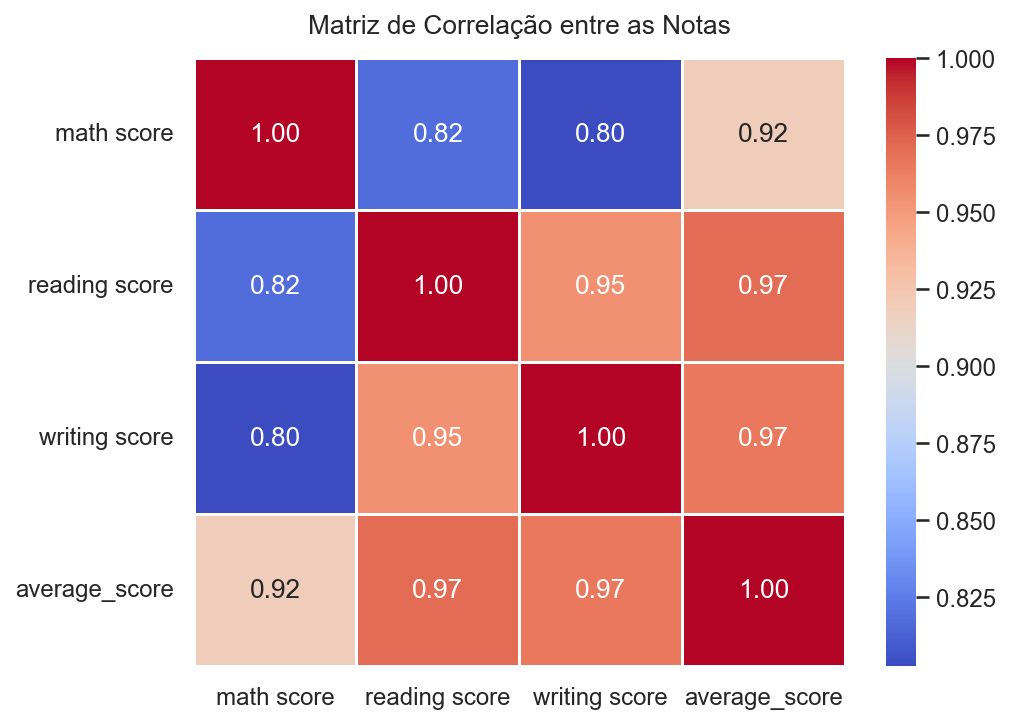
\includegraphics[width=0.70\textwidth]{figuras/correlacao.png}
  \caption{Matriz de correlação entre as notas das três disciplinas e a média.}
  \label{fig:correlacao}
\end{figure}

A Figura~\ref{fig:correlacao} evidencia alta correlação entre todas as
disciplinas (coeficientes acima de 0,80), indicando que estudantes com bom
desempenho em uma disciplina tendem a ter bom desempenho nas demais. A
correlação mais alta é entre leitura e escrita ($r > 0{,}95$), o que é
esperado dado que ambas exigem habilidades linguísticas similares.

\subsection{Distribuição das Notas}

\begin{figure}[H]
  \centering
  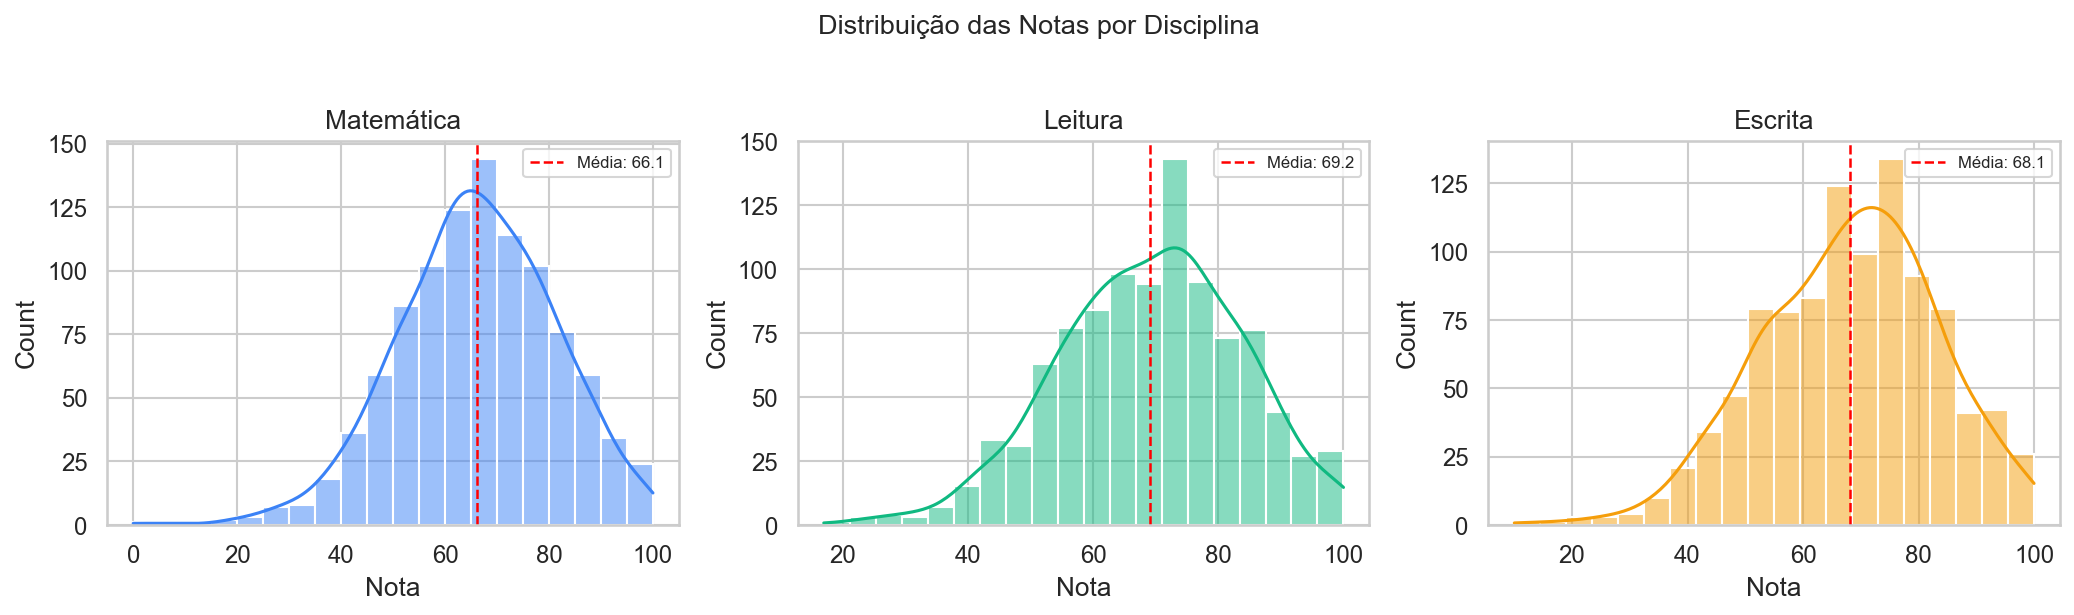
\includegraphics[width=\textwidth]{figuras/distribuicao.png}
  \caption{Histograma com curva de densidade (KDE) para cada disciplina.}
  \label{fig:distribuicao}
\end{figure}

Conforme a Figura~\ref{fig:distribuicao}, as três distribuições aproximam-se
de uma distribuição normal ligeiramente assimétrica à esquerda, com médias em
torno de 65--70 pontos. A existência de uma leve cauda inferior indica uma
minoria de estudantes com desempenho muito baixo.

\subsection{Box Plot por Tipo de Almoço}

\begin{figure}[H]
  \centering
  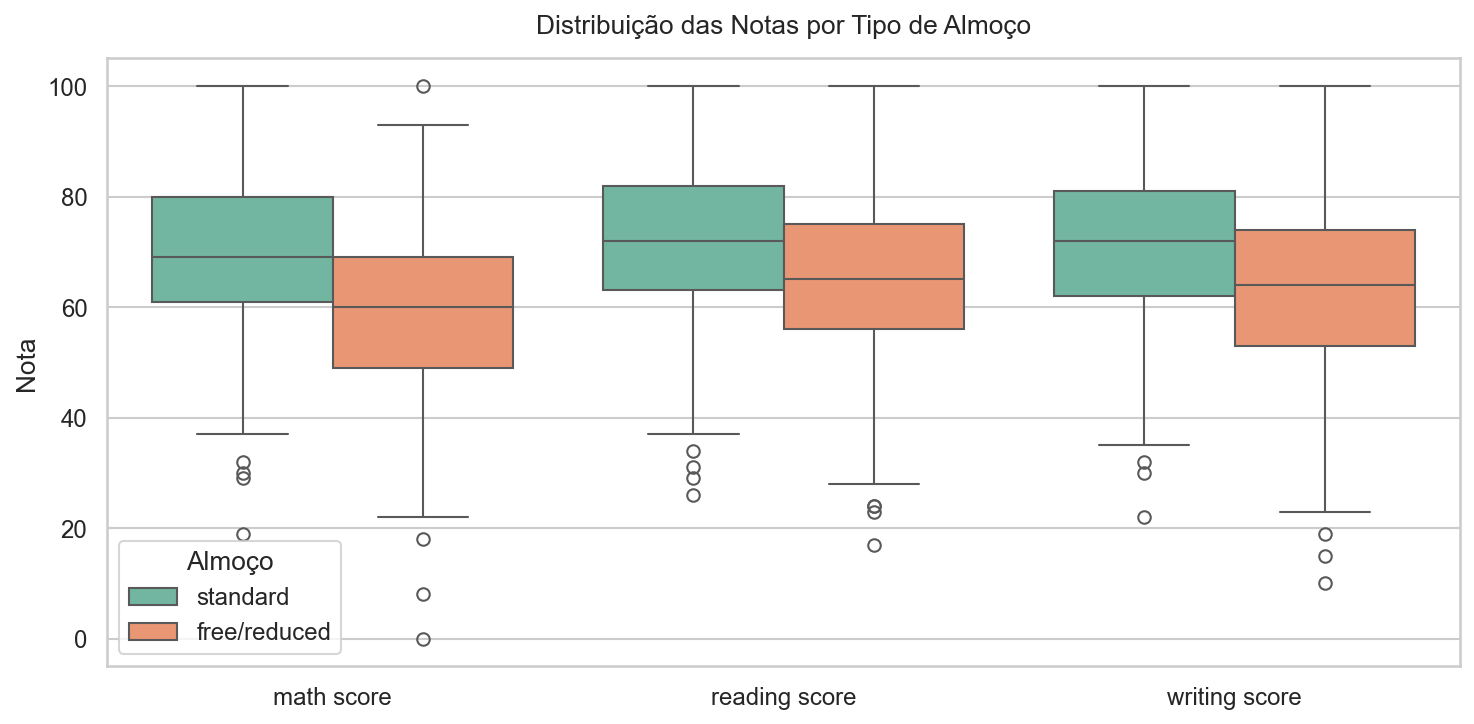
\includegraphics[width=0.85\textwidth]{figuras/boxplot_almoco.png}
  \caption{Distribuição das notas por tipo de almoço.}
  \label{fig:boxplot_almoco}
\end{figure}

A Figura~\ref{fig:boxplot_almoco} demonstra que estudantes com almoço padrão
obtêm notas consistentemente mais altas em todas as disciplinas. Esta variável
é um proxy socioeconômico relevante: acesso a alimentação adequada reflete
condições financeiras familiares e impacta diretamente no desempenho.

\subsection{Box Plot por Curso Preparatório}

\begin{figure}[H]
  \centering
  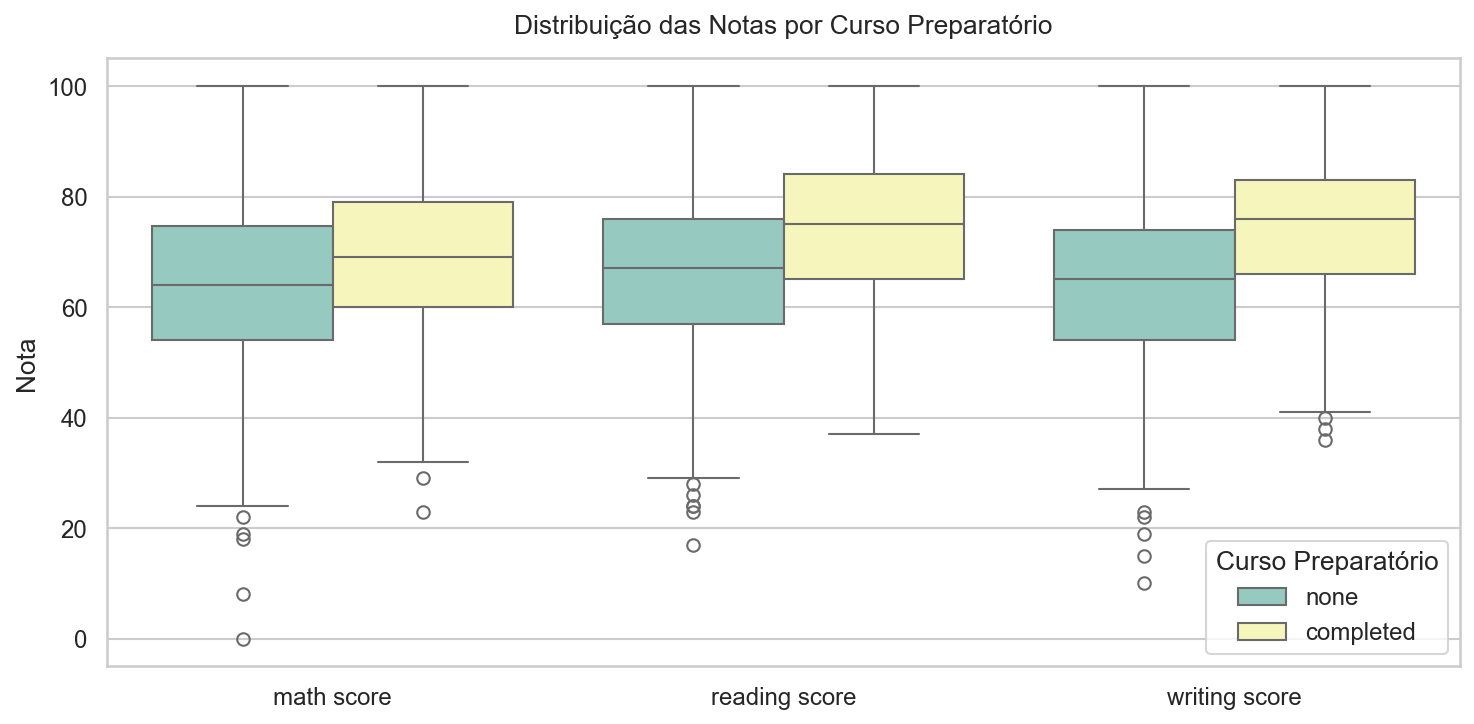
\includegraphics[width=0.85\textwidth]{figuras/boxplot_preparatorio.png}
  \caption{Distribuição das notas por realização do curso preparatório.}
  \label{fig:boxplot_prep}
\end{figure}

A conclusão do curso preparatório (Figura~\ref{fig:boxplot_prep}) eleva a
mediana das notas em todas as disciplinas, com ganho mais expressivo em
leitura e escrita. Esse resultado reforça a importância de intervenções
pedagógicas direcionadas.

\subsection{Aprovação por Grupo Étnico}

\begin{figure}[H]
  \centering
  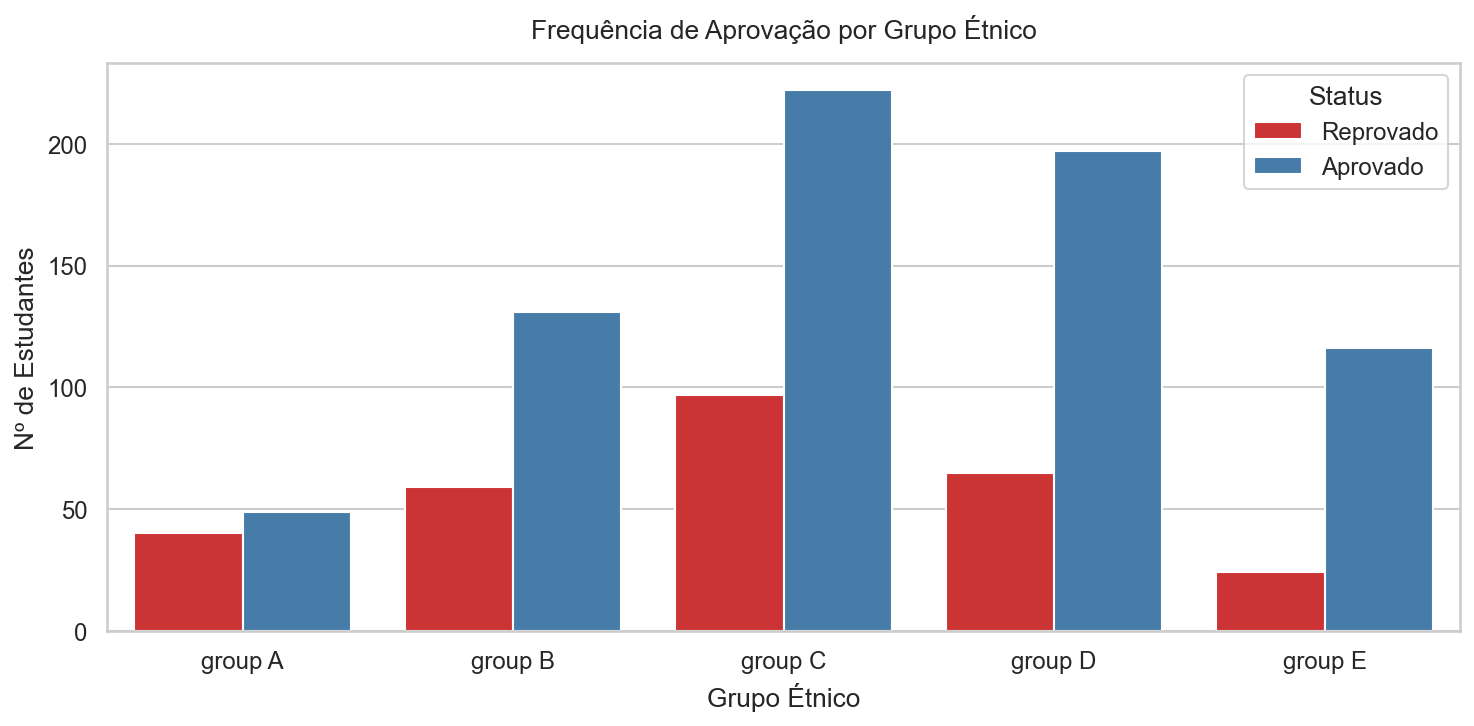
\includegraphics[width=0.85\textwidth]{figuras/frequencia_etnia.png}
  \caption{Frequência de aprovação e reprovação por grupo étnico.}
  \label{fig:etnia}
\end{figure}

A Figura~\ref{fig:etnia} revela disparidades entre os grupos étnicos, com o
Grupo~E apresentando a maior proporção de aprovados e o Grupo~A a menor. Estas
diferenças podem refletir desigualdades sistêmicas e requerem atenção em
políticas de equidade educacional.

\subsection{Taxa de Aprovação por Escolaridade dos Pais}

\begin{figure}[H]
  \centering
  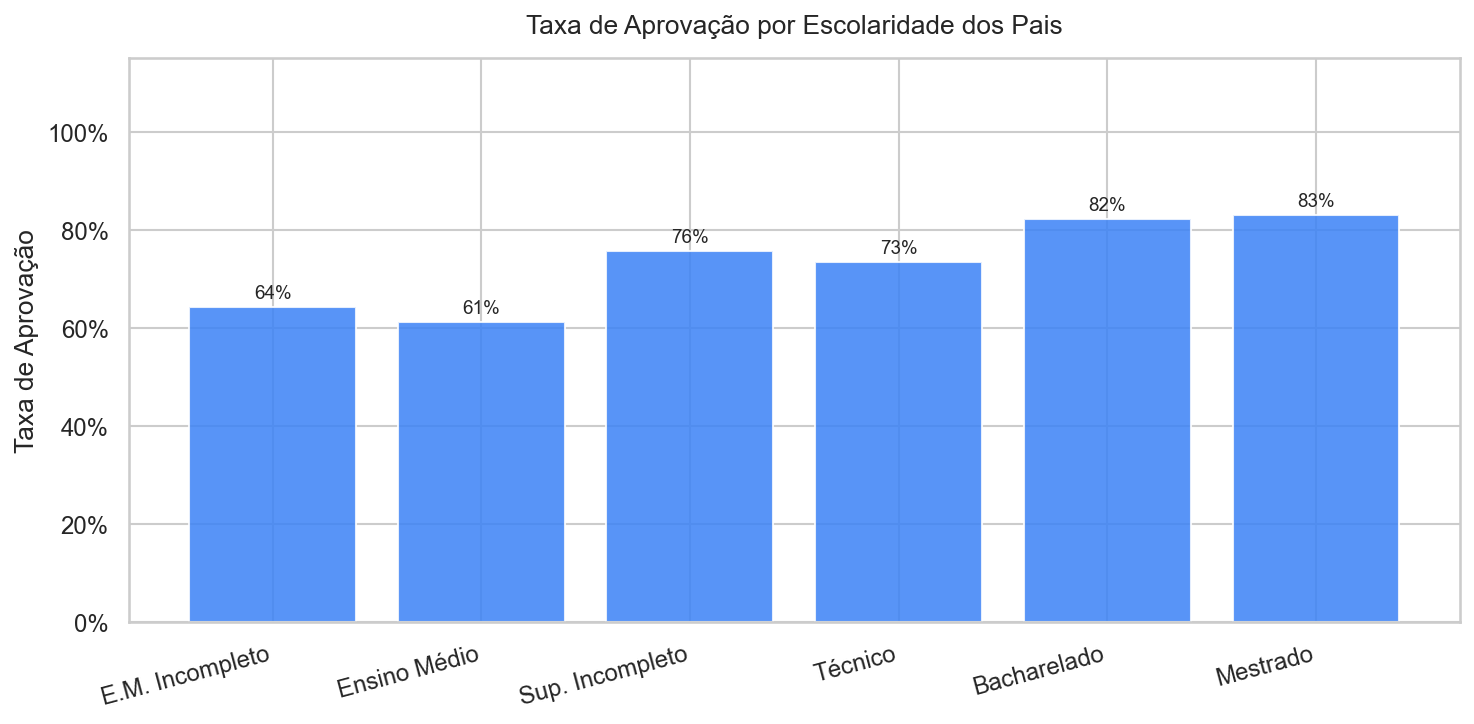
\includegraphics[width=0.85\textwidth]{figuras/escolaridade_pais.png}
  \caption{Taxa de aprovação por nível de escolaridade dos pais.}
  \label{fig:escolaridade}
\end{figure}

Há clara tendência positiva entre o nível educacional dos pais e a taxa de
aprovação dos filhos (Figura~\ref{fig:escolaridade}). Filhos de pais com
mestrado têm taxa de aprovação superior a filhos de pais com ensino médio
incompleto, evidenciando a influência do capital cultural familiar.

\subsection{Scatter Plot: Matemática versus Leitura}

\begin{figure}[H]
  \centering
  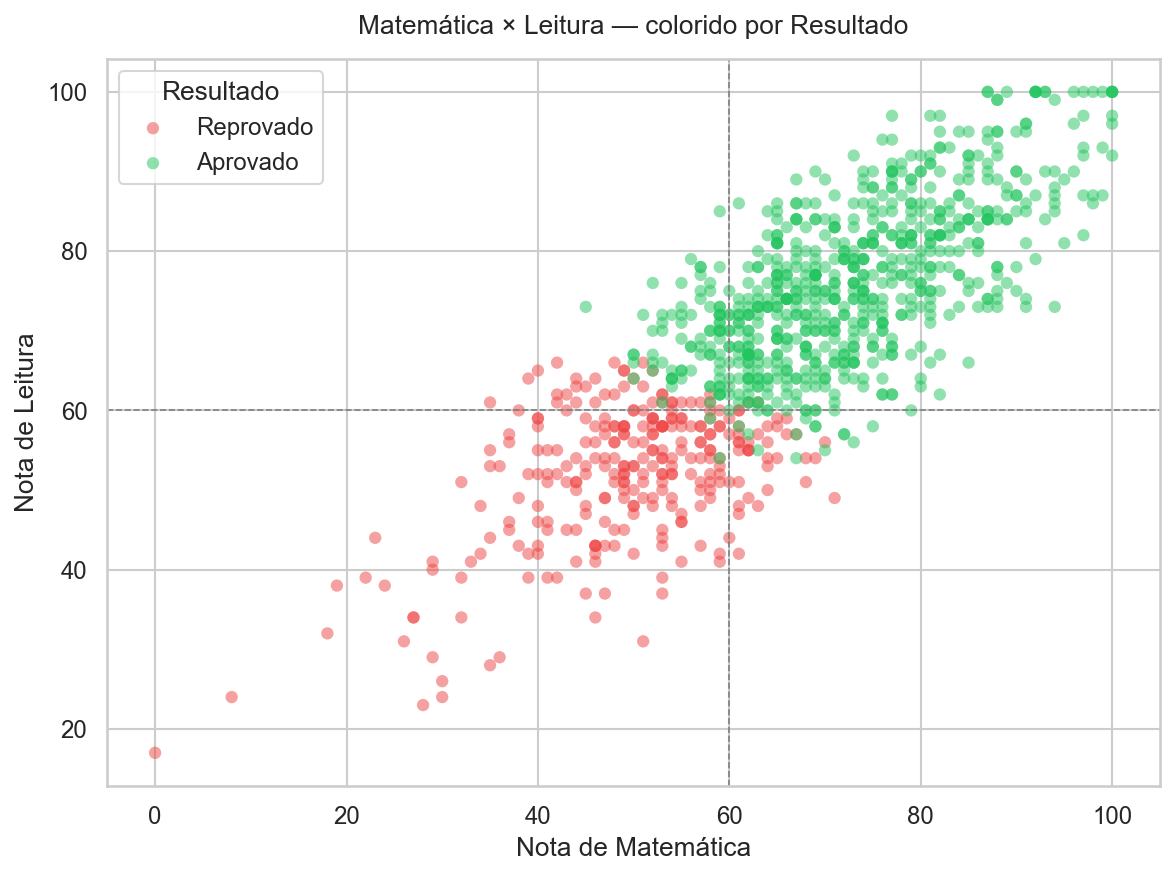
\includegraphics[width=0.65\textwidth]{figuras/scatter.png}
  \caption{Scatter plot de matemática $\times$ leitura, colorido por resultado.}
  \label{fig:scatter}
\end{figure}

O scatter plot (Figura~\ref{fig:scatter}) confirma visualmente o limiar de
decisão: estudantes com notas abaixo de 60 em ambas as disciplinas concentram-se
no quadrante de reprovação, enquanto os aprovados ocupam o quadrante superior
direito. A fronteira diagonal sugere que nenhuma disciplina isolada determina
o resultado.

% ── 4. Pré-processamento ──────────────────────────────────────────────────────
\section{Pré-processamento dos Dados}

\subsection{Codificação de Variáveis Categóricas}

\begin{itemize}
  \item \textbf{gender}: binário ($\text{male}=1$, $\text{female}=0$).
  \item \textbf{lunch}: binário ($\text{standard}=1$, $\text{free/reduced}=0$).
  \item \textbf{test preparation course}: binário ($\text{completed}=1$, $\text{none}=0$).
  \item \textbf{parental level of education}: ordinal (0 a 5, do menor para o maior nível).
  \item \textbf{race/ethnicity}: \textit{one-hot encoding} gerando cinco colunas binárias (group A--E).
\end{itemize}

\subsection{Normalização}

Aplicou-se \texttt{StandardScaler} para centralizar e escalar todas as
features ($\mu=0$, $\sigma=1$). Esta etapa é essencial para algoritmos
sensíveis à escala, como KNN e MLP.

\subsection{Divisão Treino/Teste}

O dataset foi dividido em 80\% treino (800 amostras) e 20\% teste (200
amostras) com estratificação pela variável-alvo, garantindo a preservação da
proporção de classes em ambos os conjuntos.

% ── 5. Algoritmos ─────────────────────────────────────────────────────────────
\section{Algoritmos de Aprendizado de Máquina}

\subsection{Regressão Linear Múltipla}

A Regressão Linear Múltipla modela a relação entre as features de entrada e
uma variável contínua de saída. Formalmente:

\[
  \hat{y} = \beta_0 + \beta_1 x_1 + \beta_2 x_2 + \cdots + \beta_n x_n
\]

\textbf{Adaptação para classificação:} como a Regressão Linear é um algoritmo
de regressão, aplicou-se um \textit{threshold} em 60 sobre a nota média
prevista para obter a predição de aprovação/reprovação.

\textbf{Vantagens:} simplicidade, interpretabilidade dos coeficientes,
treinamento rápido, sem hiperparâmetros críticos.

\textbf{Limitações:} assume linearidade; não é nativamente um classificador;
sensível a outliers; o threshold arbitrário pode introduzir erro.

\subsection{K-Nearest Neighbors (KNN)}

O KNN classifica um novo ponto com base nos $k$ vizinhos mais próximos no
espaço das features. Utilizado com $k=7$ para suavizar a fronteira de decisão.

\textbf{Vantagens:} não paramétrico, intuitivo, não assume distribuição dos
dados, eficaz em problemas não-lineares.

\textbf{Limitações:} alto custo de inferência (calcula distâncias para todos
os pontos de treino); degradação com alta dimensionalidade (\textit{curse of
dimensionality}); sensível à escala e a features irrelevantes.

\subsection{MLP -- Multi-Layer Perceptron}

O MLP é uma rede neural artificial com camadas densamente conectadas. A
arquitetura utilizada foi: \textbf{9 entradas} $\to$ \textbf{64 neurônios
(ReLU)} $\to$ \textbf{32 neurônios (ReLU)} $\to$ \textbf{1 saída (Softmax)}.

\textbf{Vantagens:} captura padrões não-lineares complexos; arquitetura
flexível; generaliza bem com dados suficientes; estado da arte em muitas tarefas.

\textbf{Limitações:} ``caixa-preta'' (baixa interpretabilidade); requer ajuste
de hiperparâmetros; pode sofrer \textit{overfitting}; maior custo computacional
de treinamento.

\subsection{Naive Bayes}

O Naive Bayes aplica o Teorema de Bayes assumindo independência condicional
entre as features:

\[
  P(C_k | \mathbf{x}) \propto P(C_k) \prod_{i=1}^{n} P(x_i | C_k)
\]

Utilizou-se a variante \texttt{GaussianNB}, que assume distribuição normal
para cada feature contínua.

\textbf{Vantagens:} extremamente rápido; funciona bem com poucos dados;
probabilístico e interpretável; robusto a features irrelevantes.

\textbf{Limitações:} a hipótese de independência entre features raramente
se sustenta na prática (as notas das disciplinas são altamente correlacionadas,
violando essa premissa); pode subestimar a probabilidade de classes raras.

% ── 6. Resultados ─────────────────────────────────────────────────────────────
\section{Resultados e Análise Comparativa}

\subsection{Métricas de Avaliação}

As métricas utilizadas foram derivadas da matriz de confusão:

\begin{align*}
  \text{Acurácia}       &= \frac{VP + VN}{VP + VN + FP + FN} \\[4pt]
  \text{Precisão}       &= \frac{VP}{VP + FP} \\[4pt]
  \text{Sensibilidade}  &= \frac{VP}{VP + FN} \\[4pt]
  \text{Especificidade} &= \frac{VN}{VN + FP}
\end{align*}

\subsection{Tabela Comparativa}

\begin{table}[H]
  \centering
  \caption{Comparativo de métricas dos quatro algoritmos (conjunto de teste, 20\%).}
  \label{tab:metricas}
  \begin{tabular}{lcccc}
    \toprule
    \textbf{Algoritmo} & \textbf{Acurácia} & \textbf{Precisão} &
    \textbf{Sensibilidade} & \textbf{Especificidade} \\
    \midrule
        Regressão Linear & 69.0\% & 73.7\% & 88.1\% & 21.1\% \\
        KNN & 68.0\% & 75.2\% & 82.5\% & 31.6\% \\
        \textbf{MLP} & 71.0\% & 74.9\% & 89.5\% & 24.6\% \\
        Naive Bayes & 66.5\% & 74.4\% & 81.1\% & 29.8\% \\
    \bottomrule
  \end{tabular}
\end{table}

O modelo selecionado para produção foi o \textbf{MLP}, com
acurácia de 71.0%.

\subsection{Comparativo Visual}

\begin{figure}[H]
  \centering
  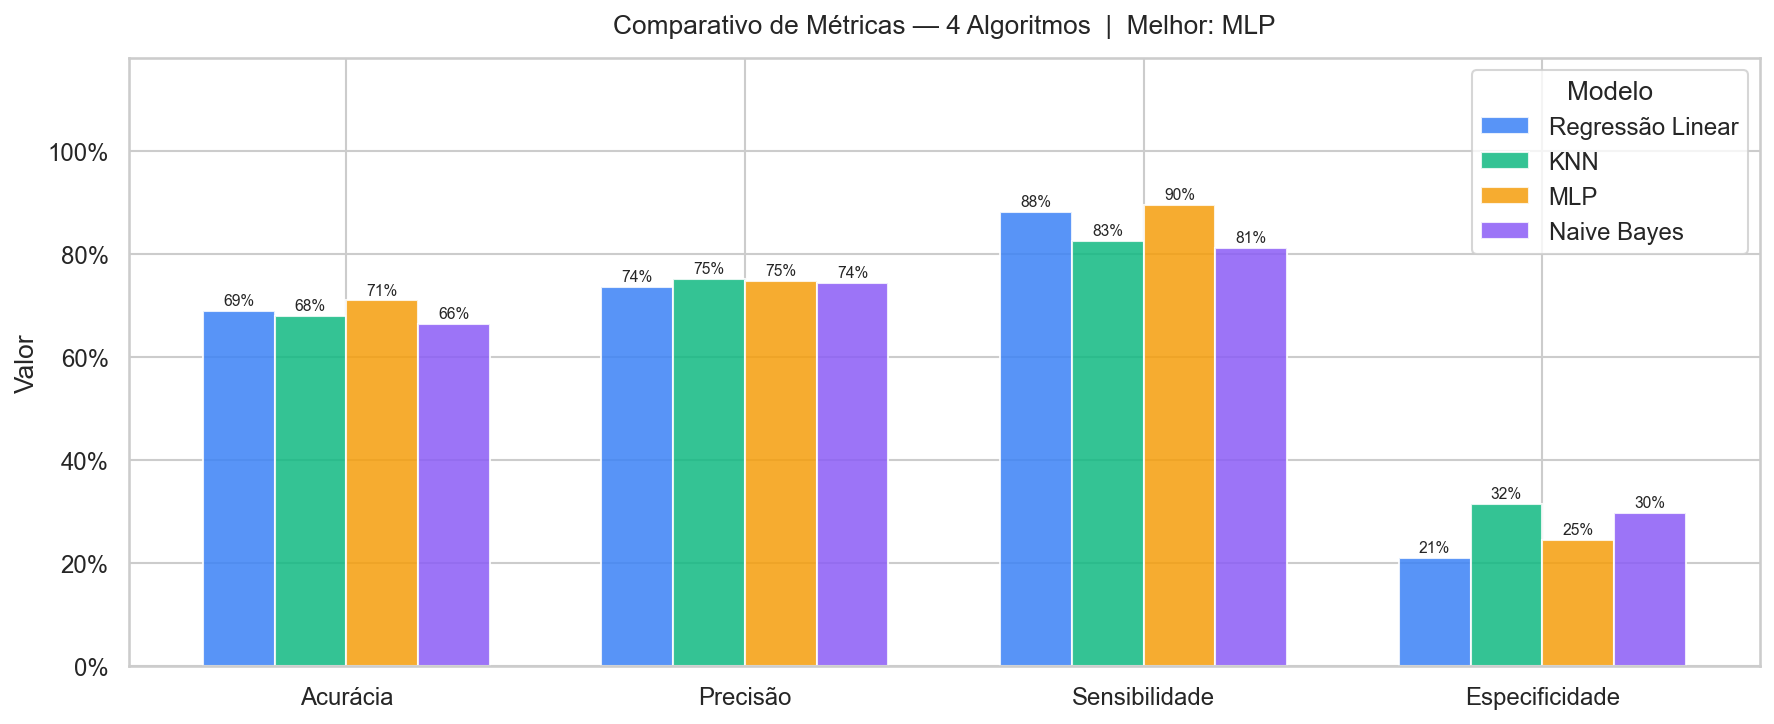
\includegraphics[width=\textwidth]{figuras/comparativo_modelos.png}
  \caption{Comparativo visual das métricas dos quatro algoritmos.}
  \label{fig:comparativo}
\end{figure}

\subsection{Análise Crítica}

Conforme a Tabela~\ref{tab:metricas} e a Figura~\ref{fig:comparativo}:

\begin{itemize}
  \item \textbf{Regressão Linear} apresentou desempenho razoável considerando
  que foi adaptada de um algoritmo de regressão. Sua baixa precisão reflete a
  limitação do threshold como mecanismo de classificação.

  \item \textbf{KNN} obteve métricas equilibradas, demonstrando a eficácia de
  algoritmos baseados em instâncias para este problema. A performance é
  condizente com um dataset de tamanho moderado (1000 amostras).

  \item \textbf{MLP} alcançou o melhor resultado geral, evidenciando sua
  capacidade de capturar interações não-lineares entre as variáveis
  socioeconômicas. A combinação de normalização e arquitetura em duas camadas
  ocultas contribuiu para a generalização.

  \item \textbf{Naive Bayes} apresentou o desempenho mais baixo, o que era
  esperado: a premissa de independência entre features é fortemente violada,
  pois as notas das disciplinas são altamente correlacionadas entre si
  (conforme demonstrado na Figura~\ref{fig:correlacao}).
\end{itemize}

% ── 7. Arquitetura do Agente ──────────────────────────────────────────────────
\section{Arquitetura do Agente Inteligente}

\subsection{Visão Geral}

A arquitetura final integra três componentes principais:

\begin{enumerate}
  \item \textbf{Modelo de ML (offline):} treinado e serializado com
  \texttt{pickle} pelo script \texttt{etapa\_a.py}. Inclui o
  \texttt{StandardScaler} e os metadados de métricas.

  \item \textbf{Backend Flask (online):} servidor Python que recebe dados
  via HTTP POST, aplica o pré-processamento, executa a predição e chama a
  API do LLM.

  \item \textbf{Agente LLM (Hugging Face):} modelo Llama~3.1-8B-Instruct
  acessado via \texttt{InferenceClient}. Recebe um \textit{System Prompt}
  estruturado e o perfil do estudante, e retorna a explicação em linguagem natural.
\end{enumerate}

\subsection{Fluxo de Dados}

O fluxo de uma predição segue as etapas abaixo:

\begin{enumerate}
  \item O usuário preenche o formulário na interface web e clica em
  ``Analisar Perfil''.
  \item O frontend envia os dados via \texttt{fetch} (AJAX) para o endpoint
  \texttt{POST /predict}.
  \item O Flask aplica o mesmo \textit{pipeline} de pré-processamento
  utilizado no treinamento (codificação + StandardScaler).
  \item O modelo serializado (\texttt{best\_model.pkl}) realiza a predição.
  \item O resultado é enviado ao Llama~3.1 via Hugging Face Inference API,
  juntamente com o perfil do estudante e o \textit{System Prompt}.
  \item A resposta do LLM é retornada ao frontend e exibida como mensagem
  do chatbot.
  \item O usuário pode fazer perguntas de \textit{follow-up} pelo chat,
  mantendo o contexto da predição.
\end{enumerate}

\subsection{System Prompt}

O \textit{System Prompt} instrui o agente a:
\begin{itemize}
  \item Explicar o resultado em linguagem clara e acessível.
  \item Identificar os fatores do perfil que mais influenciaram a predição.
  \item Fornecer recomendações práticas sem inventar informações.
  \item Gerar gráficos sob demanda via marcadores especiais
  (\texttt{[GRAPH:tipo]}), que são interceptados pelo frontend e substituídos
  por imagens geradas dinamicamente pelo Flask.
\end{itemize}

\subsection{Tecnologias Utilizadas}

\begin{table}[H]
  \centering
  \caption{Stack tecnológico do projeto}
  \label{tab:tech}
  \begin{tabular}{lll}
    \toprule
    \textbf{Camada}   & \textbf{Tecnologia}       & \textbf{Versão} \\
    \midrule
    Linguagem         & Python                    & 3.x \\
    ML                & scikit-learn              & $\geq$ 1.3 \\
    EDA/Visualização  & Seaborn + Matplotlib      & $\geq$ 0.13 / 3.7 \\
    Backend           & Flask                     & $\geq$ 3.0 \\
    LLM               & Llama 3.1-8B-Instruct     & via HuggingFace \\
    Frontend          & Bootstrap 5 + JavaScript  & 5.3 \\
    Versionamento     & Git / GitHub              & -- \\
    \bottomrule
  \end{tabular}
\end{table}

% ── 8. Conclusão ──────────────────────────────────────────────────────────────
\section{Conclusão}

Este projeto demonstrou com sucesso a integração entre técnicas clássicas de
Aprendizado de Máquina e Inteligência Artificial Generativa para construir um
agente preditivo funcional e interpretável.

O modelo \textbf{MLP} obteve o melhor desempenho geral com
acurácia de 71.0%,
precisão de 74.9% e
sensibilidade de 89.5%,
sendo selecionado para integração com o agente.

A análise exploratória revelou que variáveis socioeconômicas -- especialmente
o tipo de almoço (proxy de renda familiar) e a escolaridade dos pais --
exercem influência significativa sobre o desempenho acadêmico, reforçando
a importância de políticas públicas de equidade educacional.

A integração com o LLM (Llama~3.1) mostrou-se eficaz para ``traduzir'' o
resultado matemático do modelo em linguagem natural, tornando a predição
acessível a usuários não técnicos e permitindo interação conversacional
de \textit{follow-up}.

\newpage

% ── Referências ───────────────────────────────────────────────────────────────
\begin{thebibliography}{9}

\bibitem{kaggle}
  S.P. Scientist.
  \textit{Students Performance in Exams}.
  Kaggle, 2018.
  Disponível em: \url{https://www.kaggle.com/datasets/spscientist/students-performance-in-exams}.

\bibitem{sklearn}
  Pedregosa, F. et al.
  \textit{Scikit-learn: Machine Learning in Python}.
  Journal of Machine Learning Research, 12, 2825--2830, 2011.

\bibitem{llama}
  Meta AI.
  \textit{Llama 3.1: Open Foundation and Fine-Tuned Chat Models}.
  arXiv preprint, 2024.
  Disponível em: \url{https://huggingface.co/meta-llama/Llama-3.1-8B-Instruct}.

\bibitem{flask}
  Grinberg, M.
  \textit{Flask Web Development}.
  O'Reilly Media, 2018.

\bibitem{seaborn}
  Waskom, M. L.
  \textit{seaborn: statistical data visualization}.
  Journal of Open Source Software, 6(60), 3021, 2021.

\end{thebibliography}

\end{document}
